\chapter{\label{chp:background}Background}
In the early days of digital hardware design, gates were designed and layout were performed manually by hand. With the rapid growth in the numbers of transistors per digital chip design, this method quickly became too time consuming and thus the need for new and more automated design methods rose. \gls{rtl} design using \gls{hdl} has long been the standard in hardware design, but with the increasing demand for low power and small area in large \gls{soc} designs with multiple billion transistors, this methodology is no longer sufficient if hardware manufacturers want to hit the window of opportunity with their state-of-the-art product.

\section{\label{sec:hls}High-Level Synthesis}

 \gls{hls} is not a new concept as it were introduced in research papers in the late 1970 and further researcehd and developed in the 1980 and early 1990s \cite{martin2009high}. The available commercial \gls{hls} tools has however not been providing the necessary performance and benefits over \gls{hdl} development for major hardware development companies to adapt this methodology until recently.

The concept of \gls{hls} is to use higher abstraction level, often a \gls{hll}, to describe the functional specification of the circuit, and then let a tool help transform this specification into hardware represented as a \gls{rtl} or \gls{hdl}-model from the given target architectural models and design constraints. The typical \gls{hls}-flow is shown in figure \ref{fig:hlsflow} and each of the transition-steps is described in the below subsections. The input libraries contain information on available hardware resources with power, area and delay models for the target architecture.

\begin{figure}[hbpt]
\centering
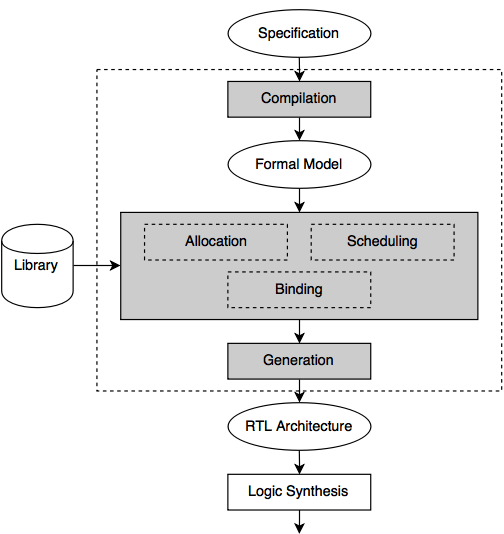
\includegraphics[width=0.6\textwidth]{../figs/HLSFlow.png}
\caption{\label{fig:hlsflow}Information flow in a typical \gls{hls} tool}
\end{figure}

\subsubsection{Compilation}

The first step of \gls{hls} is to compile the \gls{hll} into a formal model, often called an \gls{ir}. This model can vary between different tools, and can be either a specific representation language or a graphic representation of the flow. The formal model is decided by the developers of the \gls{hls} tool. 

\subsubsection{Allocation}

Necessary hardware resources such as functional units, storage and connectivity components needs to be selected from a given \gls{rtl} component library, in order to satisfy the specification and design constraints. Some \gls{hls} tools can also add more resources in scheduling and bind task if found necessary to meet given constraints.

\subsubsection{Scheduling}
Scheduling arranges all operations in an optimized sequence so that variables are read from sources and brought to the input of the correct functional unit for execution and to the destination afterwards. The scheduler takes all dependencies into account when scheduling the operations, in order to get the best most effective result, as some operations can be executed in parallel, if no dependencies exist and there is available resources. Operations can be scheduled to finish in one or take multiple clock-cycles and operations can also be chained to eliminate the need for storing the result between operations and to reduce the total number of cycles needed. 

\subsubsection{Binding}

In the binding task, all clock-cycle crossing variables, operations and transfers are bound to a free resource in the timeframe when they are scheduled. Non-overlapping or mutually exclusive variables can be bound to the the same storage unit, and operations can be bound to the best optimized functional unit if multiple alternatives are available. Each transfer from component to component, that being either storage or functional unit, needs to be bound to a connection unit, such as a bus or a multiplexer.

\subsubsection{RTL Generation}

The generated \gls{rtl} usually consists of two parts, a control unit and a data path unit. The control unit is often implemented as a \gls{fsm} that sets control signals to the data path, and controls the current and next-state of the system. The data path contains storage , functional and connection units. Depending on the intensiveness of the binding step, the output \gls{rtl} can be tightly or loosely bound to the available resources. If an operation is not bound to a specific unit, it is up to the following logic synthesis of the \gls{rtl} to bind the operations to available resources. The different types of \gls{rtl} output is illustrated by the example \textit{a = b * c} executing in state \textit{n} as follows:\\
\\
Without any binding:\hfill\vspace{-\baselineskip}
\begin{verbatim}
state (n): a = b * c;
go to state (n + 1);
\end{verbatim}
With storage binding:\hfill\vspace{-\baselineskip}
\begin{verbatim}
state (n): S(1) = S(2) * S(3);
go to state (n + 1);
\end{verbatim}
With functional-unit binding:\hfill\vspace{-\baselineskip}
\begin{verbatim}
state (n): a = MUL1 (b, c);
go to state (n + 1);
\end{verbatim}
With storage and functional-unit binding:\hfill\vspace{-\baselineskip}
\begin{verbatim}
state (n): S(1)=MUL1 (S(2), S(3));
go to state (n + 1);
\end{verbatim}\\
\clearpage
With storage, functional-unit, and connectivity binding:\hfill\vspace{-\baselineskip}
\begin{verbatim}
state (n): BUS1 = S(2); BUS2 = S(3);
BUS3 = MUL1 (BUS1, BUS2);
S(1) = BUS3;
go to state (n + 1);
\end{verbatim}
A loosely bound \gls{rtl} gives the synthesis the flexibility to optimize the unit binding to updates timing estimates and delays and loads given by the layout and floor-planning.

\section{LegUp}

The \gls{hls} tool used in this project is called LegUp \cite{canis2011legup}. LegUp is an open-source academic tool developed at the University of Toronto, Canada. LegUp's goal is to \textit{"allow researchers to experiment with new \gls{hls} algorithms without building a new infrastructure from scratch"} and their long-term vision is to \textit{"make \gls{fpga} programming easier for software developers"}. LegUp takes \acrshort{ansi} C as input and generates synthesizable Verilog \gls{hdl} as output. The developers of LegUp has primarily focused on support for a variety of \gls{fpga} boards from manufacturer Altera, but in the latest version (4.0), beta support for Xilinx devices and possibility to configure the tool to generate generic Verilog to target other \gls{fpga} vendors or even \gls{asic} through use of generic dividers, has been introduced. The big advantage of LegUp compared to similar, commercial tools is that it's open-source and thus can be configured to target different architectures and the \gls{rtl} and \gls{hdl} generating part of the framework can be modified or replaced to fit the programmers needs.

LegUp is a target back-end pass to the \gls{llvm} compiler infrastructure (described in section \ref{sec:LLVM}).
The information flow in LegUp, shown in figure \ref{fig:legupflow}, follows the same principle as the information flow described in section \ref{sec:hls} 

\begin{figure}[hbpt]
\centering
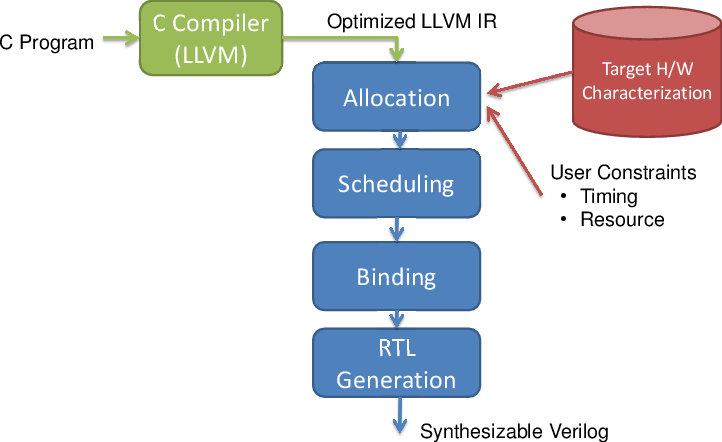
\includegraphics[width=0.6\textwidth]{../figs/LegUpFlow.png}
\caption{\label{fig:legupflow}Information flow in LegUp}
\end{figure}

\subsubsection{Producing Verilog Output}

\section{\label{sec:LLVM}LLVM}

\gls{llvm} is a compiler framework developed to handle the increasing demand for reconfigurable cross-language, cross-platform, cross-architecture compilators needed for future hw/sw codesign.

LLVM was originally developed as a research infrastructure to investigate dynamic compilation techniques for static and dynamic programming languages.

\section{Tool-flow}

After generation of Verilog, the tool flow will be adapted from the work by Joar Talstad in his specialization project \cite{talstad14powest} to estimate power and area usage. This will not be the main objective of this report.

\section{Power-estimation}

The 

\section{Area-estimation}


%2.1 High-Level Synthesis
%High-level synthesis (HLS) is a compilation technique that transforms a software behavioural description into a hardware circuit description with equivalent functionality [10]. It is sometimes referred to as behavioural synthesis or C-to-gates synthesis, as HLS often uses ANSI C/C++/SystemC (or even Java) as it input. The HLS flow is traditionally divided into four different steps [23]: allocation, scheduling, binding, and RTL generation. Allocation decides how much resources are needed in hardware and binding map the instructions and variables to hardware components, such as adders, multipliers, and registers. Scheduling divides the software behaviour into control steps which are used to define the states in a finite state machine (FSM). Each control step contains a small section of code that can be executed in a single clock cycle in hardware. Scheduling also optimizes the number of execution steps based on limits of hardware resource and cycle time. RTL generation creates HDL code based on the previous steps. The generated HDL can then be synthesized to a hardware circuit by a logic synthesis tool. The goal of HLS is to allow developers to describe their designs using a higher level of abstraction, similar to the flow used in the design of software programs.

%Figure 2.1: The Clang front end and LegUp synthesis flow.

%2.2 LegUp
%The debugging framework in this thesis is built within a larger project called LegUp \cite{canis2011legup}. LegUp is an open source high-level synthesis tool being developed at the University of Toronto. The LegUp framework allows researchers to improve C-to-Verilog synthesis without building an infrastructure from scratch. Its long-term vision is to make hardware for FPGAs the produces good results using a software-like flow. LegUp uses the Low-Level Virtual Machine (LLVM) compiler framework. It is the same framework used by Apple for iOS development. LLVM uses an intermediate representation (IR), which is an assembly-like machine independent language. LegUp utilizes Clang to compile C/C++ code into the LLVM IR. Clang is an open source compiler front end for C, C++ and Objective-C. It offers a replacement for the GNU Compiler Collection (GCC) that translates source code languages to an intermediate representation (IR). Later, the LLVM IR is translated into RTL using various optimization passes. Figure 2.1 shows the synthesis flow of LegUp. The goal of this project is to generate input circuits for this flow at the LLVM IR level which enables improved testing of the compiler optimization and LegUp synthesis steps in the flow. 

%2.3 LLVM Intermediate Representation 
%LLVM is a compiler infrastructure written in C++ [3]. It provides a framework with a complete compiler system, taking intermediate representation (IR) code as its input from a compiler front end and producing an optimized IR. This optimized IR can then be translated and linked in machine-specific assembly code for a target platform (e.g. MIPS, x86). LLVM can accept the IR from the GCC tool chain or Clang (used by LegUp), which allows different compilers to be used with LLVM. LLVM IR [3] uses static single assignment (SSA) form that provides type safety, low-level operations, flexibility, and the capability of representing high-level languages clearly. It is the common code representation used throughout all phases of the LLVM compilation strategy. It is often written in a file with a .ll file extension. In the case of LegUp, compilation starts from the LLVM IR level and takes these .ll files as its input.